\providecommand{\thebibpath}{..}
\makeatletter\def\input@path{{\thebibpath/}{.}}\makeatother
\documentclass[main.tex]{subfiles}
\begin{document}

In the process of setting up and running experiments, various electrical concerns were found - some pre-emptively, and others post-hoc. The robot uses a Lithium Polymer battery, a type for which electrical mistakes can be catastrophic\footnote{An example being the newsworthy \cite{bbc-samsung-explosion} issues with the Galaxy Note 7} - making it important to avoid mistakes, and if they are made, preventing them being repeated. In line with the risk assessment, a fire-safe battery storage bag was purchased for the project.

The simplest of these was the connection of the battery to the robot, which was made using an unpolarized and uninsulated connector, show in \cref{fig:connectors}. A similar connector was used to charge the robot. Misconnecting either of these would result in outcomes ranging from a destroyed microcontroller to an exploding battery. Having exposed connections on loose flexible wires entails similar risk. These were replaced with JST RCY connectors.

Another issue with LiPo batteries, thankfully without safety ramifications, is over-discharging them. The protection circuits within the battery cause it to enter a `sleep mode' \cite{lipo-sleep-mode}, from which it cannot be restored without a more advanced charger. After being caught out by the first battery entering this state, a battery monitor was purchased (visible in \cref{fig:robot-back}), which gives a voltage readout, and an audible alarm whenever the battery needs charging.

\begin{figure}
	\centering
	\includegraphics[width=\linewidth]{figures/electronic-back.png}
	\caption{The back of the robot}
	\label{fig:robot-back}
	\medskip
	\small
	Showing the battery monitor, a button to interact with the embedded software, and velcro battery strap
	(replacing previous duct tape).
\end{figure}

\begin{figure}
	\begin{minipage}[t]{0.45\linewidth}
		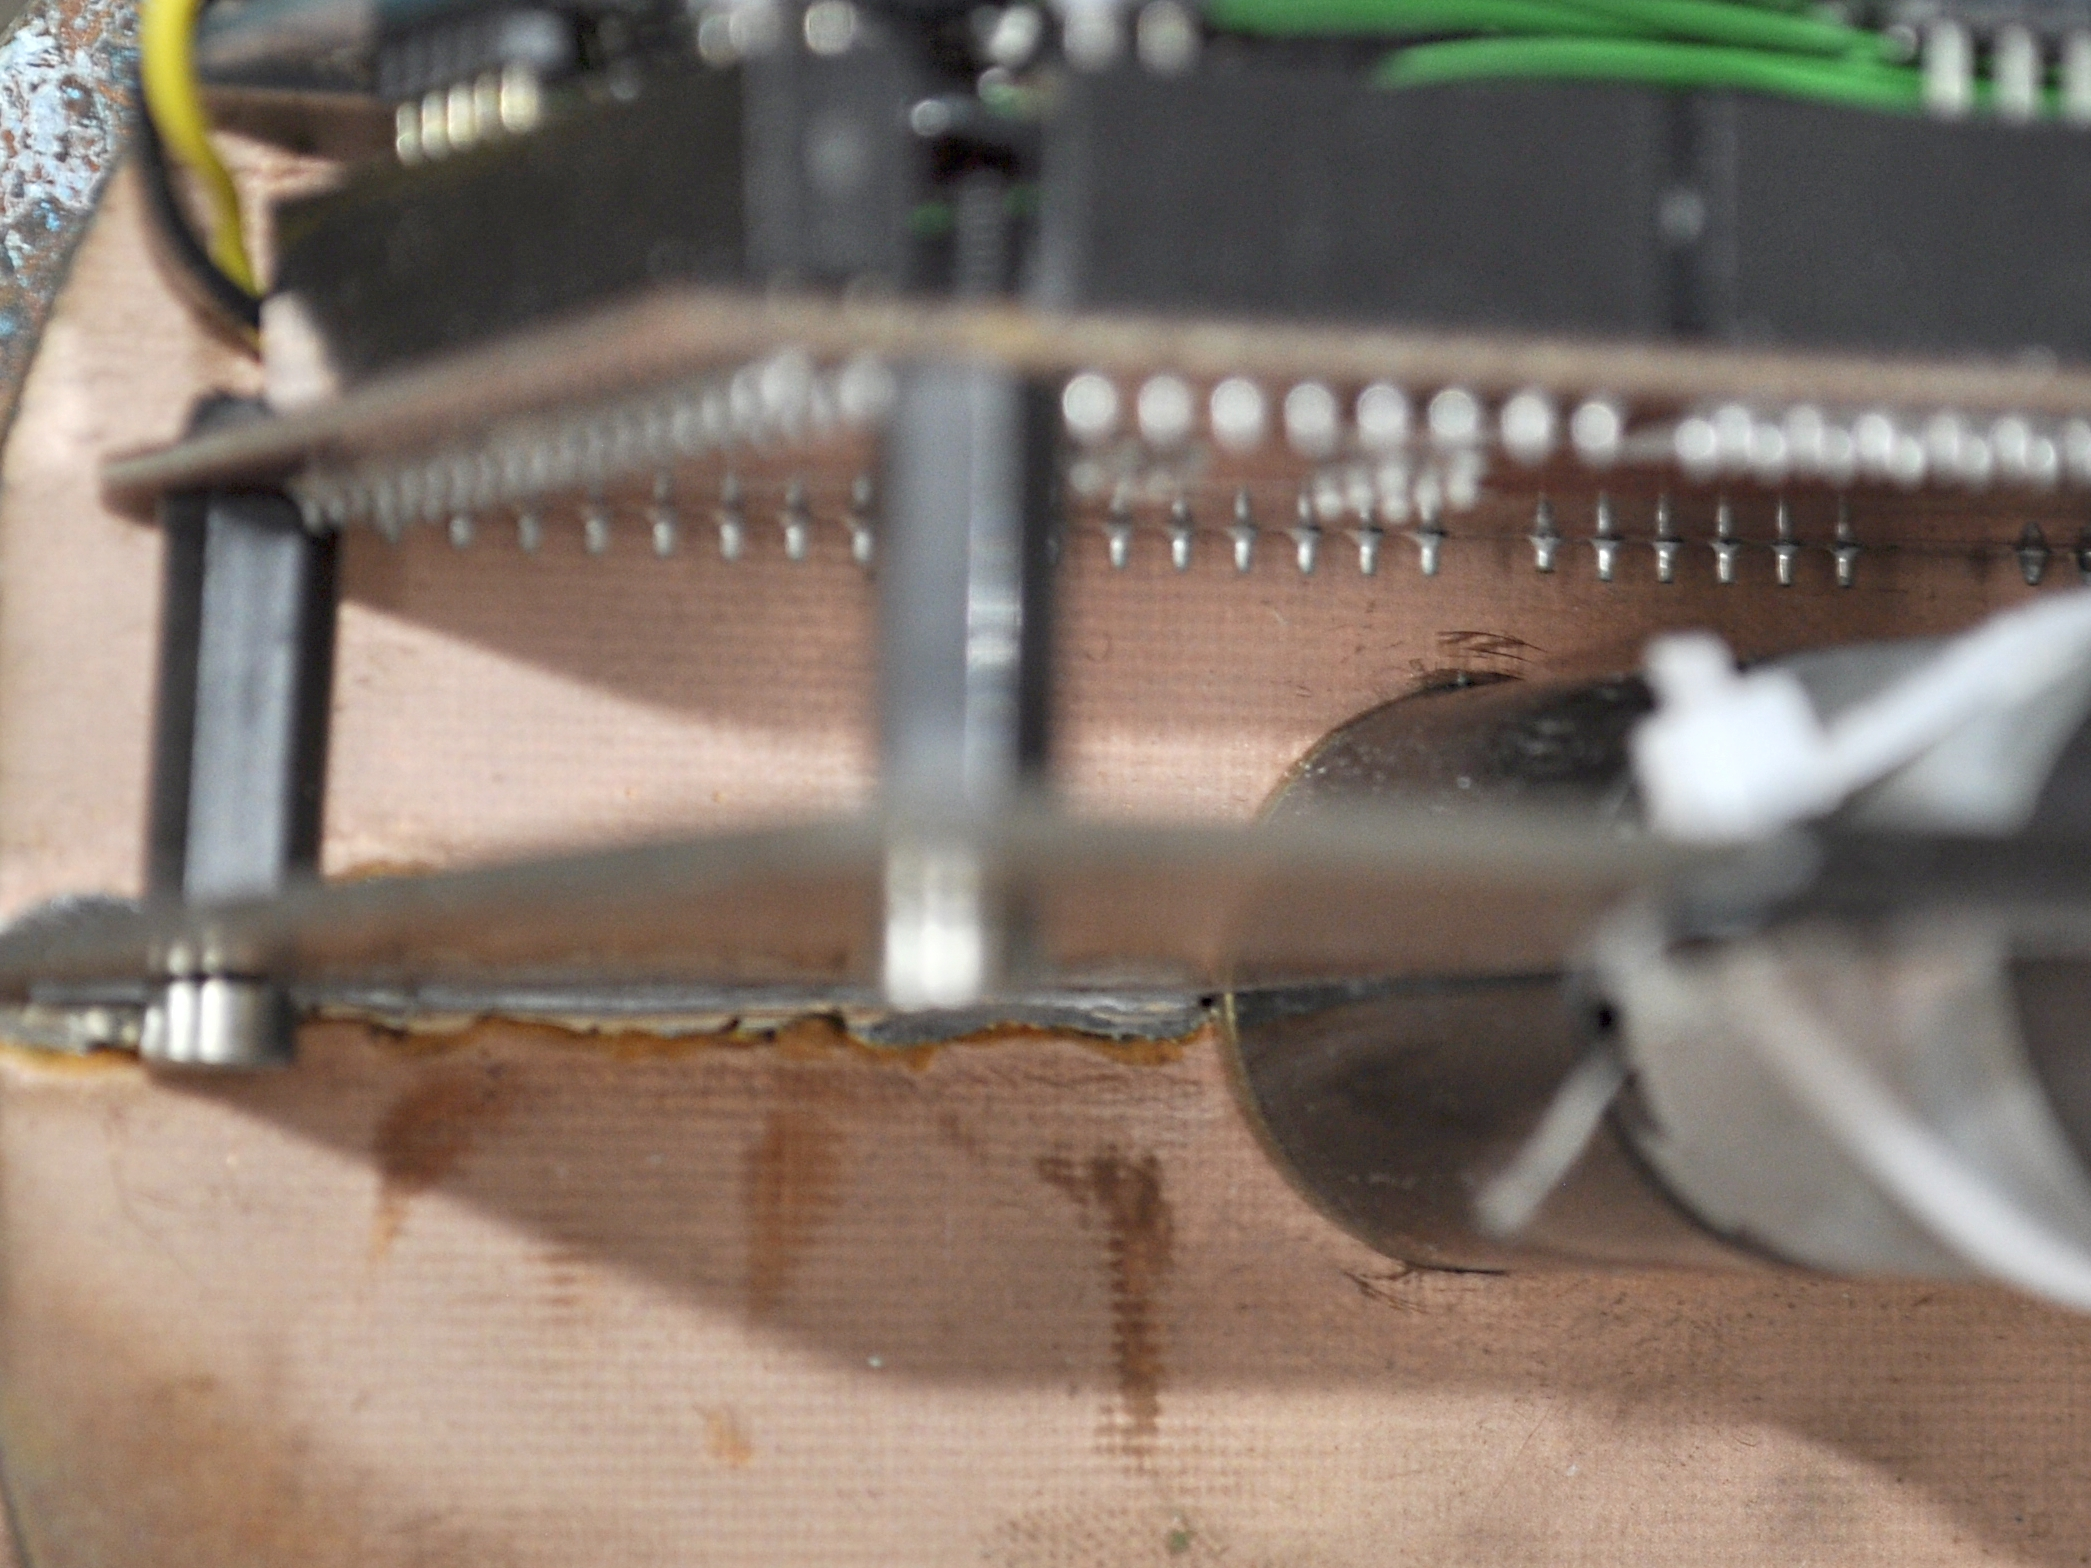
\includegraphics[width=\linewidth]{figures/standoffs.jpg}
		\caption{Clearance below controller}
		\label{fig:clearance}
		\medskip
		\small
		The black nylon standoffs replace the old metal screws. There is now a
		clear gap between the motor (right) and the pins, preventing shorts.
	\end{minipage}
	\hfill
	\begin{minipage}[t]{0.45\linewidth}
		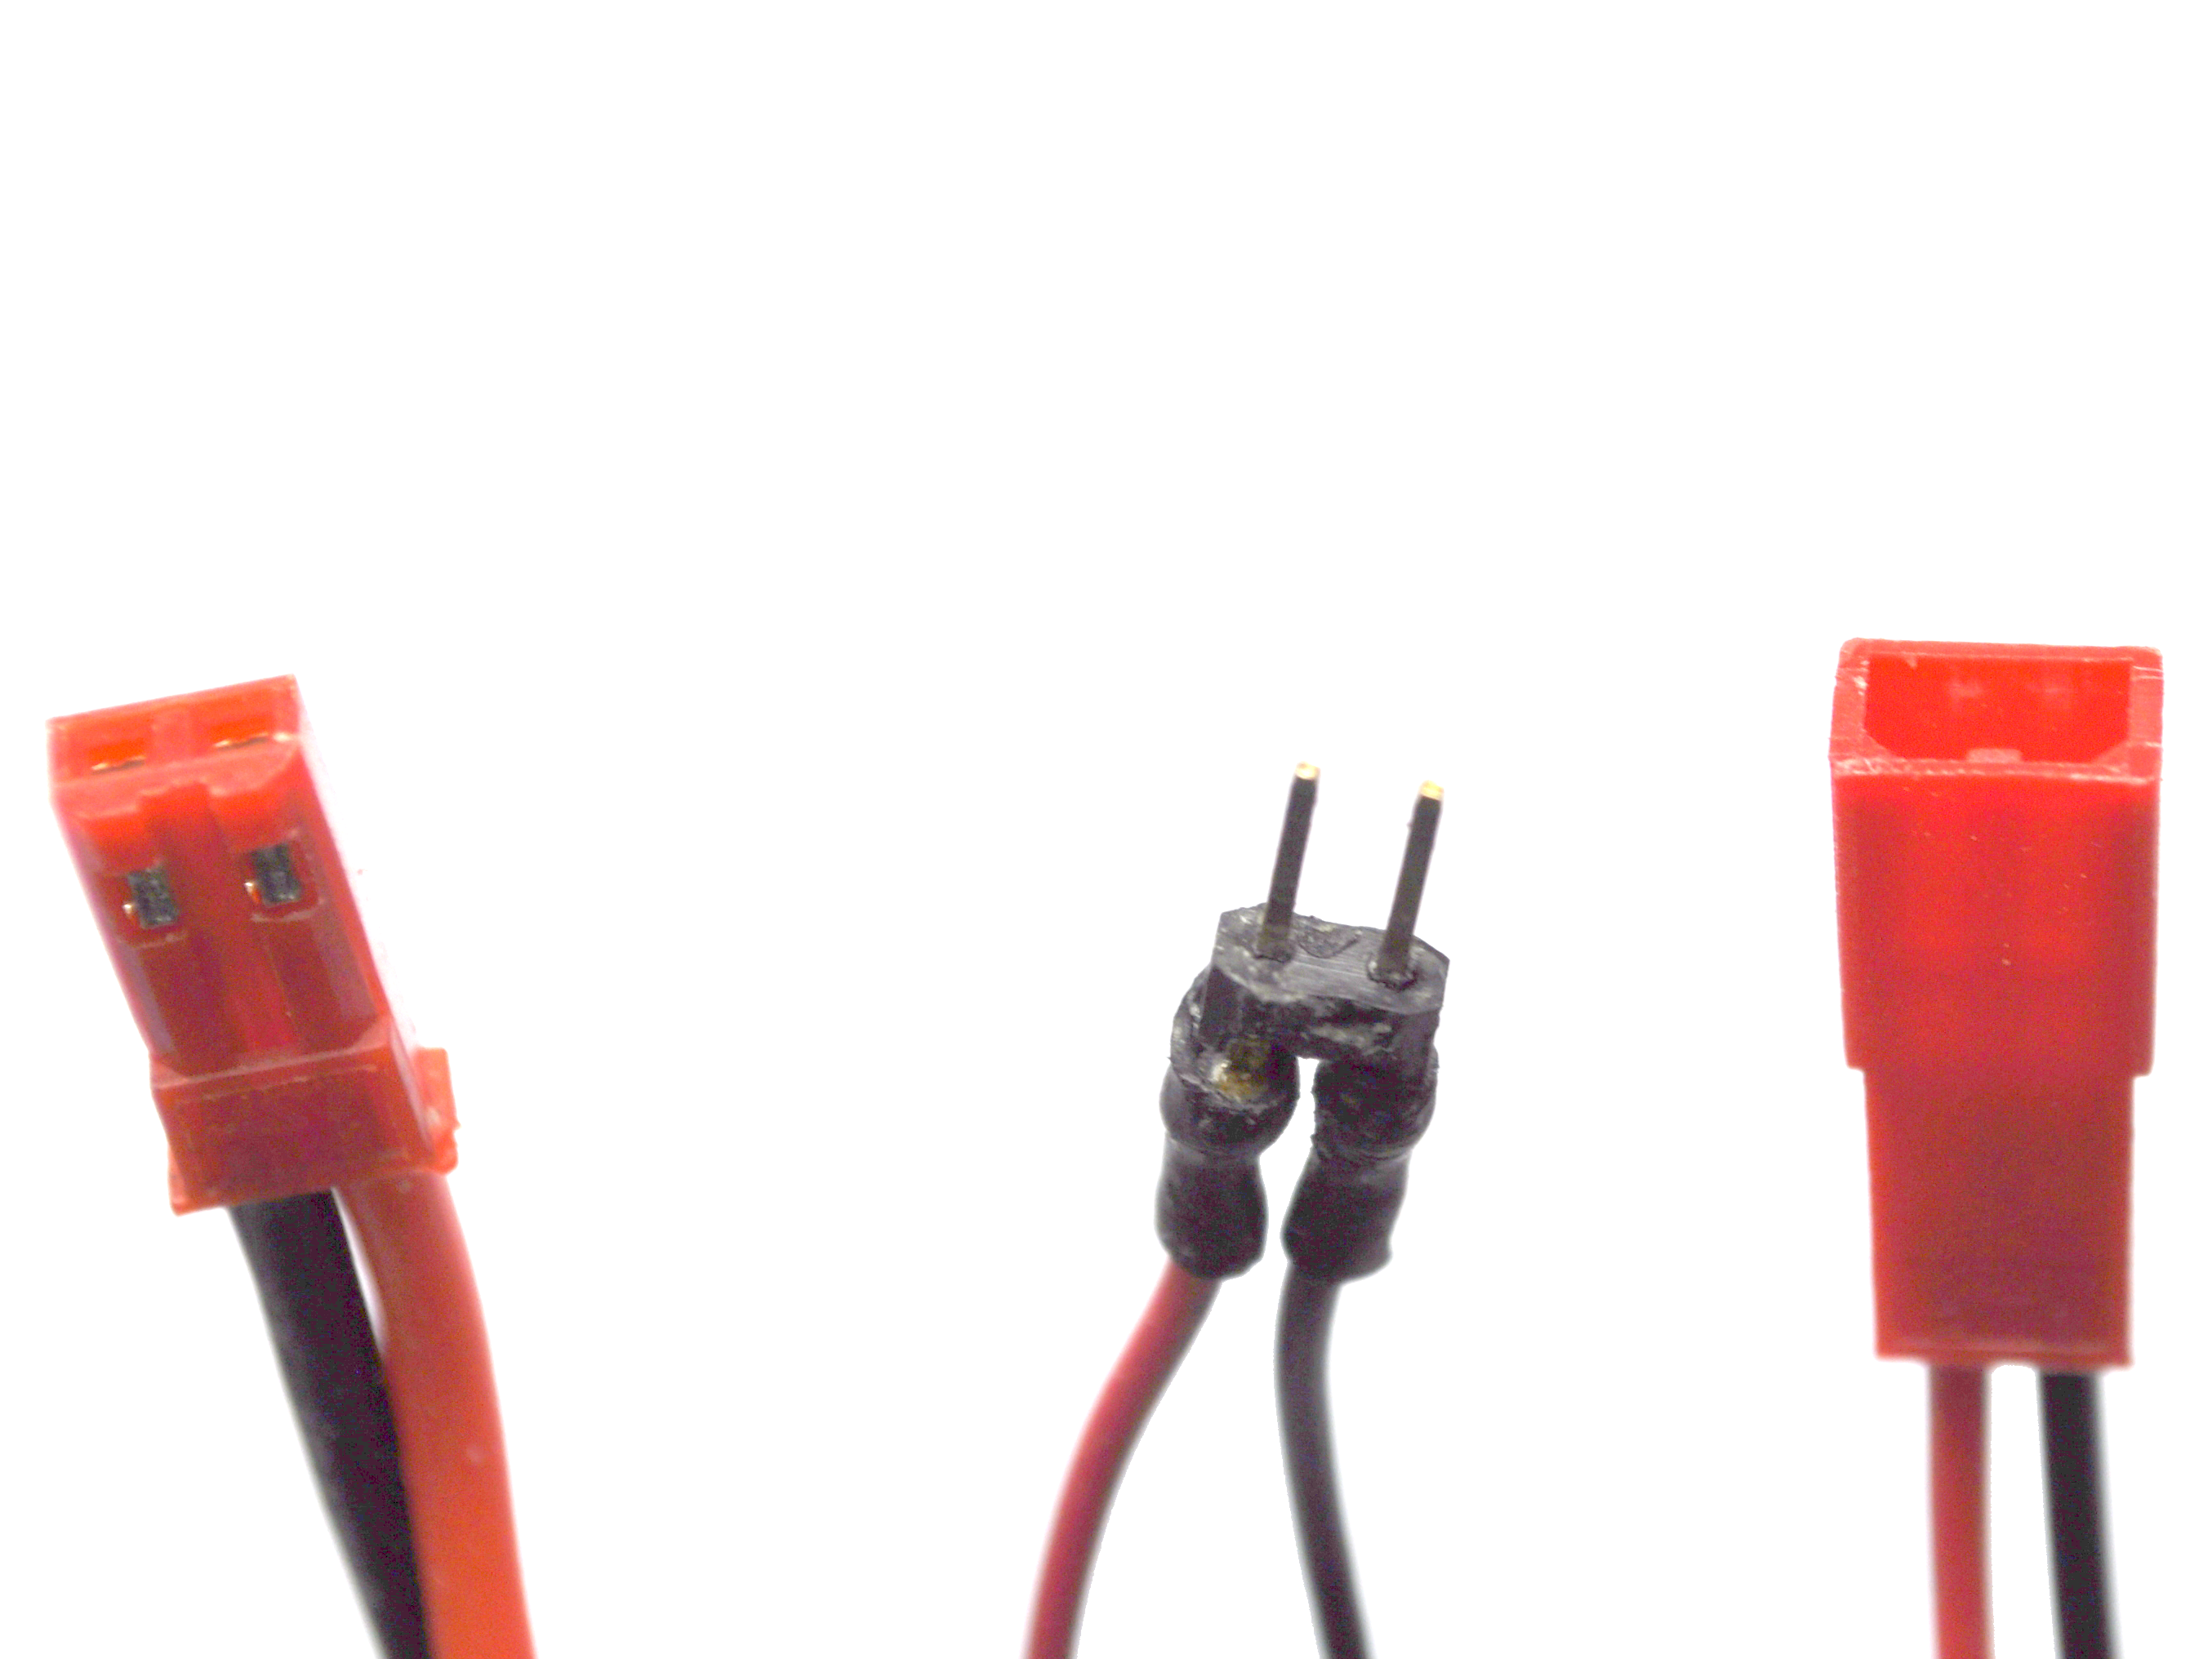
\includegraphics[width=\linewidth]{figures/battery-connectors.png}
		\caption{The power connectors}
		\label{fig:connectors}
		\medskip
		\small
		From left to right: female (battery), male unpolarized (old), male polarized (new)
	\end{minipage}
\end{figure}

\subsection{Enabling untethered operation}
	\label{sec:untethered}

	Previous data collection from the small robot required the USB cable to be connected while the robot is in motion. Cables are stiff, and thus the force from flexing them can have a considerable effect on the dynamics of an small and unstable robot -- especially with an unpredicable human holding the other end. This unpredictability is the key issue - since this cable is in a different place each time, and that information is not available to the controller, PILCO is not able to learn to handle it.

	This was not a deliberate choice -- the design of the microcontroller board makes it impossible to reattach a USB cable without resetting the microchip, as the RS232 \texttt{DTR} line is connected to the microcontroller reset\footnotemark. The solution was to cut a jumper pad on the microcontroller to break this connection, preventing this restart. This allows the USB cable to be reconnected after a test, and data to be recovered.

	\footnotetext{The RS232 protocol includes two flow control lines -- \texttt{DTR}, and \texttt{CTS}. The arduino bootloader uses both of these to allow reprogramming over USB. Unfortunately, \texttt{DTR} is unconditionally asserted by the RS232 over serial operating system driver, causing the unwanted reset. Were \texttt{CTS} used instead, there would be no problem.}

\subsection{Improving the release procedure}

	The previous approach to starting the test runs was to wait a short amount of time, and then turn on an LED.
	The operator had to time their release of the robot to match this LED, which introduces a short period of artificial stability at the start of each test run due to human reaction time (as high as \SI{300}{\milli\second}, based on a self test).

	An initial attempt was made to use an audio signal instead produced by the turntable motor, noting that human reaction time to audio is \SI{15}{\percent} faster than that to visual \cite{reaction}.
	Furthermore, by sending out a rhythmic sequence, this can be much further reduced by taking advantage of our ability to anticipate the next beat in a sequence.

	While this proved somewhat successful, a simpler approach was settled: using a limit switch, shown in \cref{fig:robot-back}.
	This is placed such that the switch is naturally pressed while holding the robot, and so the act of releasing the robot also release the switch.
	This is also used as a stop button, to terminate a rollout early once it has fallen over, or if something goes wrong.

\subsection{Electrical failure}

	During one test of the hardware, the robot began to emit smoke from a then-unidentifiable location. The priority of course was to disconnect the battery as soon as possible to prevent a fireball, but even this proved difficult, with the melting power cables giving minor burns to a finger.

	Methodical investigation followed, with the battery kept within its firesafe bag, and the entire system in a non-flammable enviroment. The process consisted of removing as much of the electronics as possible, and plugging in components one-by-one until a short was detected. This time, wire-cutters were used to break the battery connection quickly and safely when the issue arose.

	The cause is shown in \cref{TODO}. On the bottom of the microcontroller board, there is a small metal stub fastening the pin headers to the top. These stubs were being used as resting points, with one pulled against a cable tie, and the other against a painted motor. With time, the paint wore through, causing a direct short between the Vin and GND pins -- those connected directly to the battery.

	The upshot here, of course, is that the short happened through a few components as possible, with damage found only in the wiring. To prevent this issue recurring, the metal screws connecting the microcontroller to the frame were replaced with nylon standoffs (\cref{fig:clearance}) -- such that the board is now properly insulated from the frame, and furthermore has a far more rigid attachement.

	As a precaution, a 3.15A fuse was inserted into the system, such that if a short happens in future, it does so without causing damage. The rating of the fuse was chosen to be in line with the stall current of the motors \cite{motor}, making sure it did not exceed that of the 22AWG wires connecting it (roughly 5A).


% https://electronics.stackexchange.com/a/230164/1217


\bib

\end{document}
